\documentclass[12pt,a4]{article}
\usepackage{hyperref}
\usepackage{color}
\usepackage{fullpage}
\usepackage{graphicx}
\usepackage{epstopdf}	
\begin{document}

\begin{center}

\textbf{\center{\Large Predicting drug-pathway interactions using the Correlated Topic Model}}\\
A. I\v{s}kovs (\texttt{ai280@cam.ac.uk})\\
\vspace{0.3in}

Supervisor: N. Pratanwanich\\
Director of Studies: Dr~A.~C.~Norman\\
Project Overseers: Dr~A.~V.~S.~Madhavapeddy  \& Dr~S.~H.~Teuffel\\

\end{center}

% Main document

\section*{Progress report}

My project attempts to use the Correlated Topic Model, a bag-of-words topic modelling algorithm, to predict pathways that a drug may affect given its gene expression data. As part of this, I have implemented in Python the training (inference) process for the Correlated Topic Model as per the original paper this work builds up on. I extended it with a way to set topic-word membership priors and wrote a routine for generation of toy datasets. This allowed to begin the evaluation and the debugging of the model. In addition, I implemented routines to plot the resultant correlation matrices and document similarity matrices as graphs (using \texttt{GraphViz}), which allows to visualize the relationships between topics (pathways) and documents (drugs). My model was run on the real KEGG/CMap dataset and produced some promising results. The project is hence entirely on schedule.

A difficulty that I have had to overcome in evaluating the performance of the model is that of the topic identifiability. The CTM assumes that the documents are generated by first drawing a distribution of topics for every single document and then picking a topic and drawing a word from its word distribution for every word in the document. This means that the recovered topic structure is not at all guaranteed to be the same as the one used to generate the evaluation dataset, which most often manifests itself as topics being output in the wrong order. Hence, it might not be possible to distinguish between an issue in the implementation and an issue in the model itself. I am currently using topic priors to mitigate that: the entries on the diagonal of the topic-word matrix are set to zero, which enforces that for every topic, there is one word that it cannot contain. This gives a slight ``hint'' to the model about the structure of every topic and the order they should be output in. This amount of sparsity is often not sufficient and so the evaluation process also ``cheats" by considering which per-word topic distributions from the inferred and the reference topic structures are the closest and permuting the topics accordingly. While these ambiguities hinder the evaluation process, the real gene-pathway membership dataset is very sparse (each pathway has few of the overall number of genes as its members) and so I am not expecting these kinds of difficulties with real data.

Another, more expected, difficulty was the performance of Python. Since it's an interpreted language that allows high levels of abstraction (which helped me immensely during the development of the model), it is not naturally suited for numerical computations and \texttt{NumPy}, a numerical library for Python, helps with that. I used a profiler to identify performance bottlenecks in the code. These turned out to be the use of various Pythonisms like list comprehensions and explicit iterations through arrays in the variational inference loop. I made sure to rewrite all of them to matrix products that are evaluated by \texttt{NumPy}'s native code. In addition, I took advantage of the fact that the variational inference process for every document is independent by executing it in parallel for several documents at once. Using this and some other optimisations like precomputing reused values or recycling the results of variational inference by using them to initialise the function minimiser on the next iteration, the total training time for the test dataset of similar size to the KEGG/CMap datasets is about 8 hours.

I am now planning to:

\begin{itemize}
\item Continue evaluating the model using toy datasets: I have concerns that some of the model parameters (the mean and the covariance matrix of the global topic distributions) are not being recovered correctly.
\item Refactor the code and implement some unit tests.
\item Consider more performance improvements, for example, using \texttt{numexpr}, a numerical expression evaluator that compiles \texttt{NumPy} expressions into a low-level VM bytecode.
\item Start work on the dissertation and consider which extensions to the project to start implementing once the main objective has been achieved.
\end{itemize}

\begin{figure}[!htb]

\includegraphics[width=\textwidth]{progress-report-pathways.eps}
\caption{Sample graph of pathway correlations (only pathways that have correlations greater than 0.185, roughly the 99.9th percentile of all correlation values between all pairs, are plotted). The model correctly identifies phenomena such as the relation between neurodegenerative diseases (Parkinson's, Huntington's, Alzheimer's), the relation between pyrine and pyrimidine (similar molecular structures) metabolism or the association of the hedgehog signalling pathway with basal cell carcinomas.}
\end{figure}

\begin{figure}[!htb]
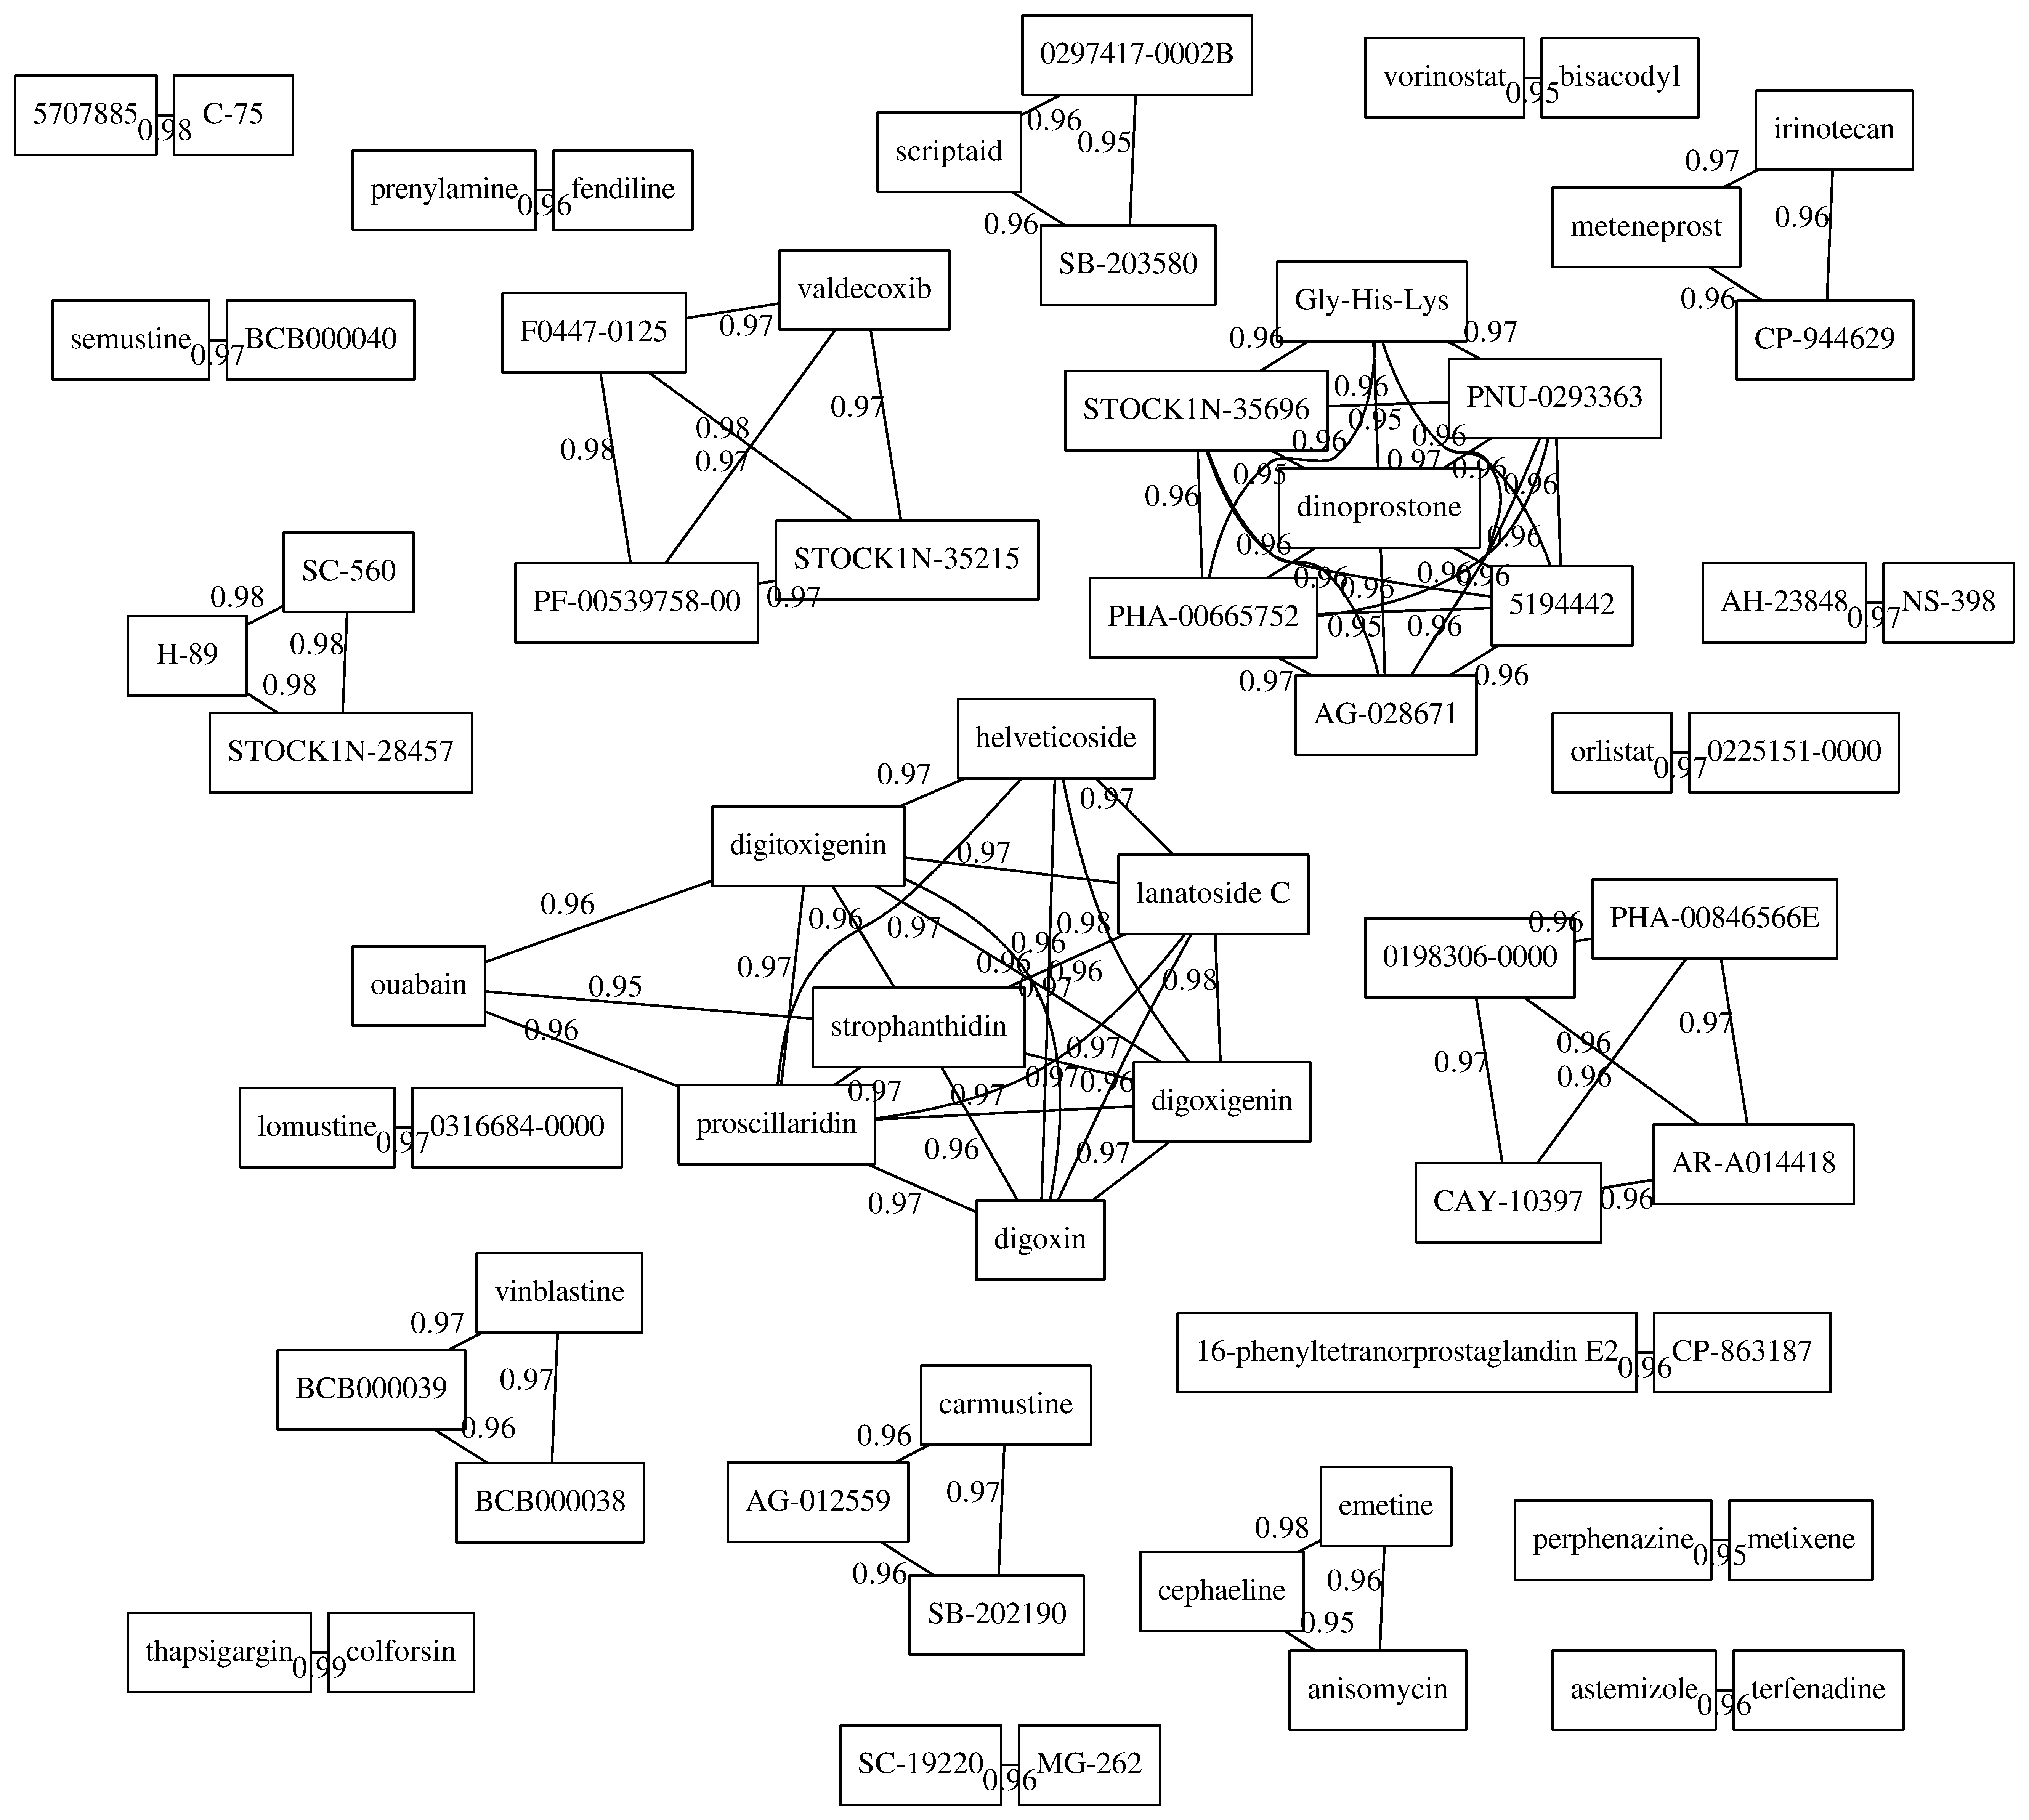
\includegraphics[width=\textwidth]{progress-report-drugs.eps}
\caption{Sample graph of the cosine similarities of drug-pathway distributions. The drugs from the sample dataset have many common pathways and so are all very similar (95\% of all drug pairs have similarity above 0.776 and 50\% above 0.877). Here, only similarities above 0.950 are plotted. Some similar drugs are identified, such as the cluster in the middle including digoxin, digoxigenin and digitoxigenin (used for cancer chemotherapy and treatment of heart conditions).}
\end{figure}

\end{document}